\lecture{2}{3 March.}{}
An arbitrary sorting algorithm is a function that takes the sequence of answers to our queries (is \(x_i < x_j\)?) and returns a permutation \(\pi \in S_n\) s.t. \(x_{\pi (1)} < x_{\pi (2)} < \dots < x_{\pi (n)}\). Suppose the algorithm has a worst-case running time of \(k\). Then this function has at most \(2^k\) different outputs since such binary decision tree can has at most \(2^k\) leaves and each leaf represent a possible permutation.

\begin{figure}[H]
    \centering
    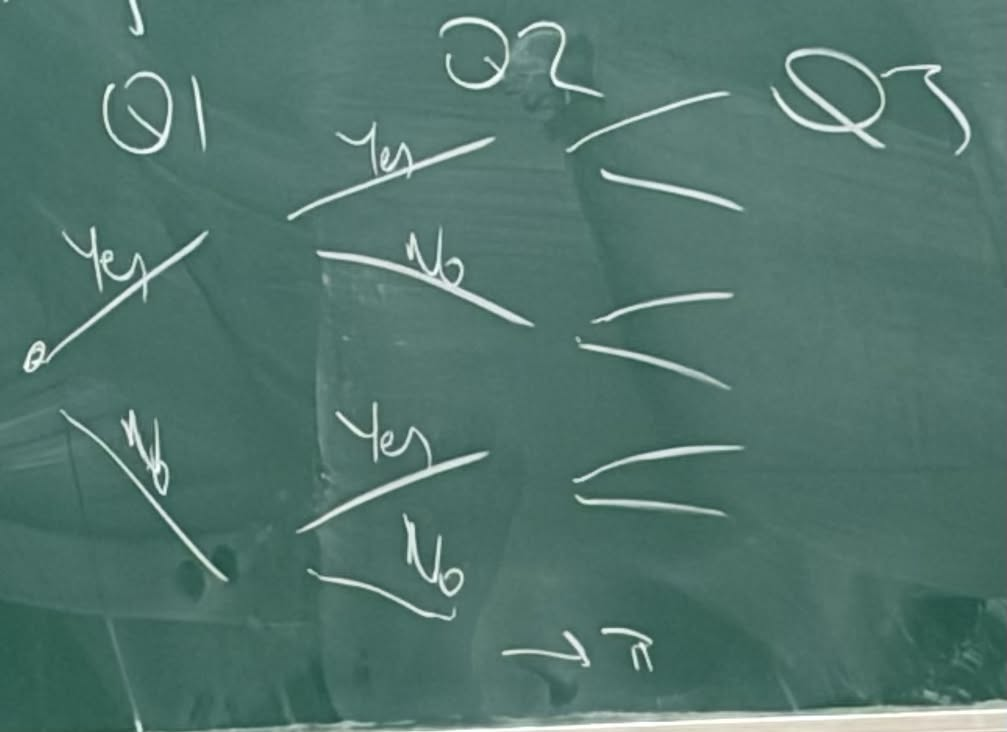
\includegraphics[width=0.3\textwidth]{./Figures/DecisionTree.jpg}
    \caption{The decision tree}
\end{figure}

The entirety of \(S_n\) has to be in the image, so \(2^k \ge \vert S_n \vert = n! \). Hence, \(k \ge \log _2 (n!) = (1 + o(1)) n \log _2 n\).  

\subsubsection{Alternative arguments (playing against the devil)}

You ask the comparisons to the devil, whose goal is to make the game go on as long as possible, The devil maintains a list of all possible permutations. Every time we do a comparison, we split the list into two: Those whose the answer is "yes" and those where it is "no". The devil chooses the answer with the bigger part. Game ends when the list has size \(1\). Let \(L_i\) be the list of possible permutations after \(i\) comparisons. \(L_0 = S_n\), and for all \(i \ge 1\), 
\[
    \vert L_i \vert \ge \frac{1}{2} \vert L_{i-1} \vert.  
\]    
Suppose one algorithm requires \(k\) comparisons in the worst case, then 
\[
    1 \ge \vert L_k \vert \ge \frac{1}{2} \vert L_{k-1} \vert \ge \frac{1}{4} \vert L_{k-2} \vert \ge \dots \ge \frac{1}{2^k} \vert L_0 \vert = \frac{n!}{2^k},   
\] 
so \(2^k \ge n!\), which shows \(k \ge (1 + o(1)) n \log _2 n\).

\chapter{Connectivity and Spanning Tree}
\begin{definition}[graph]
    A (simple) graph is an ordered pair of sets \((V, E)\), where \(V\) is a set of vertices and \(E \subseteq \binom{V}{2}\) is a set of edges, where an edge is an unordered pair of disjoint vertices.   
\end{definition}

\begin{definition}
    A walk in a graph is a sequence 
    \[
        v_0 e_1 v_1 e_2 v_2 e_3 v_3 \dots e_n v_n
    \] where \(v_i \in V\) and \(e_i = \left\{ v_{i-1}, v_i \right\}  \in E\) for all \(i\). A trail is a walk that does not repeat any edges. A path is a trail/walk without repeated vertices. A circuit is a trail that starts and ends at the same vertex. A cycle is a circuit that doesn't repeat any internal vertex.   
\end{definition}

\begin{definition}
    A graph \(G = (V, E)\) is connected if for every \(u, v \in V\), there is a path(walk) from \(u\) to \(v\).   
\end{definition}

\begin{definition}
    Given a graph \(G = (V, E)\) and a vertex \(v \in V\), the connected componnent of \(v\) is the maximal connected subgraph of \(G\) that contains \(v\).     
\end{definition}

\begin{remark}
    \(G^{\prime} = \left( V^{\prime} , E^{\prime}  \right) \) is a subgraph of \(G = (V, E)\) if \(V^{\prime} \subseteq V\) and \(E^{\prime} \subseteq E \cap \binom{V^{\prime} }{2}\). It is induced if \(E^{\prime} = E \cap \binom{V^{\prime} }{2}\). It is spanning if \(V^{\prime} = V\).       
\end{remark}

\begin{figure}[H]
    \centering
    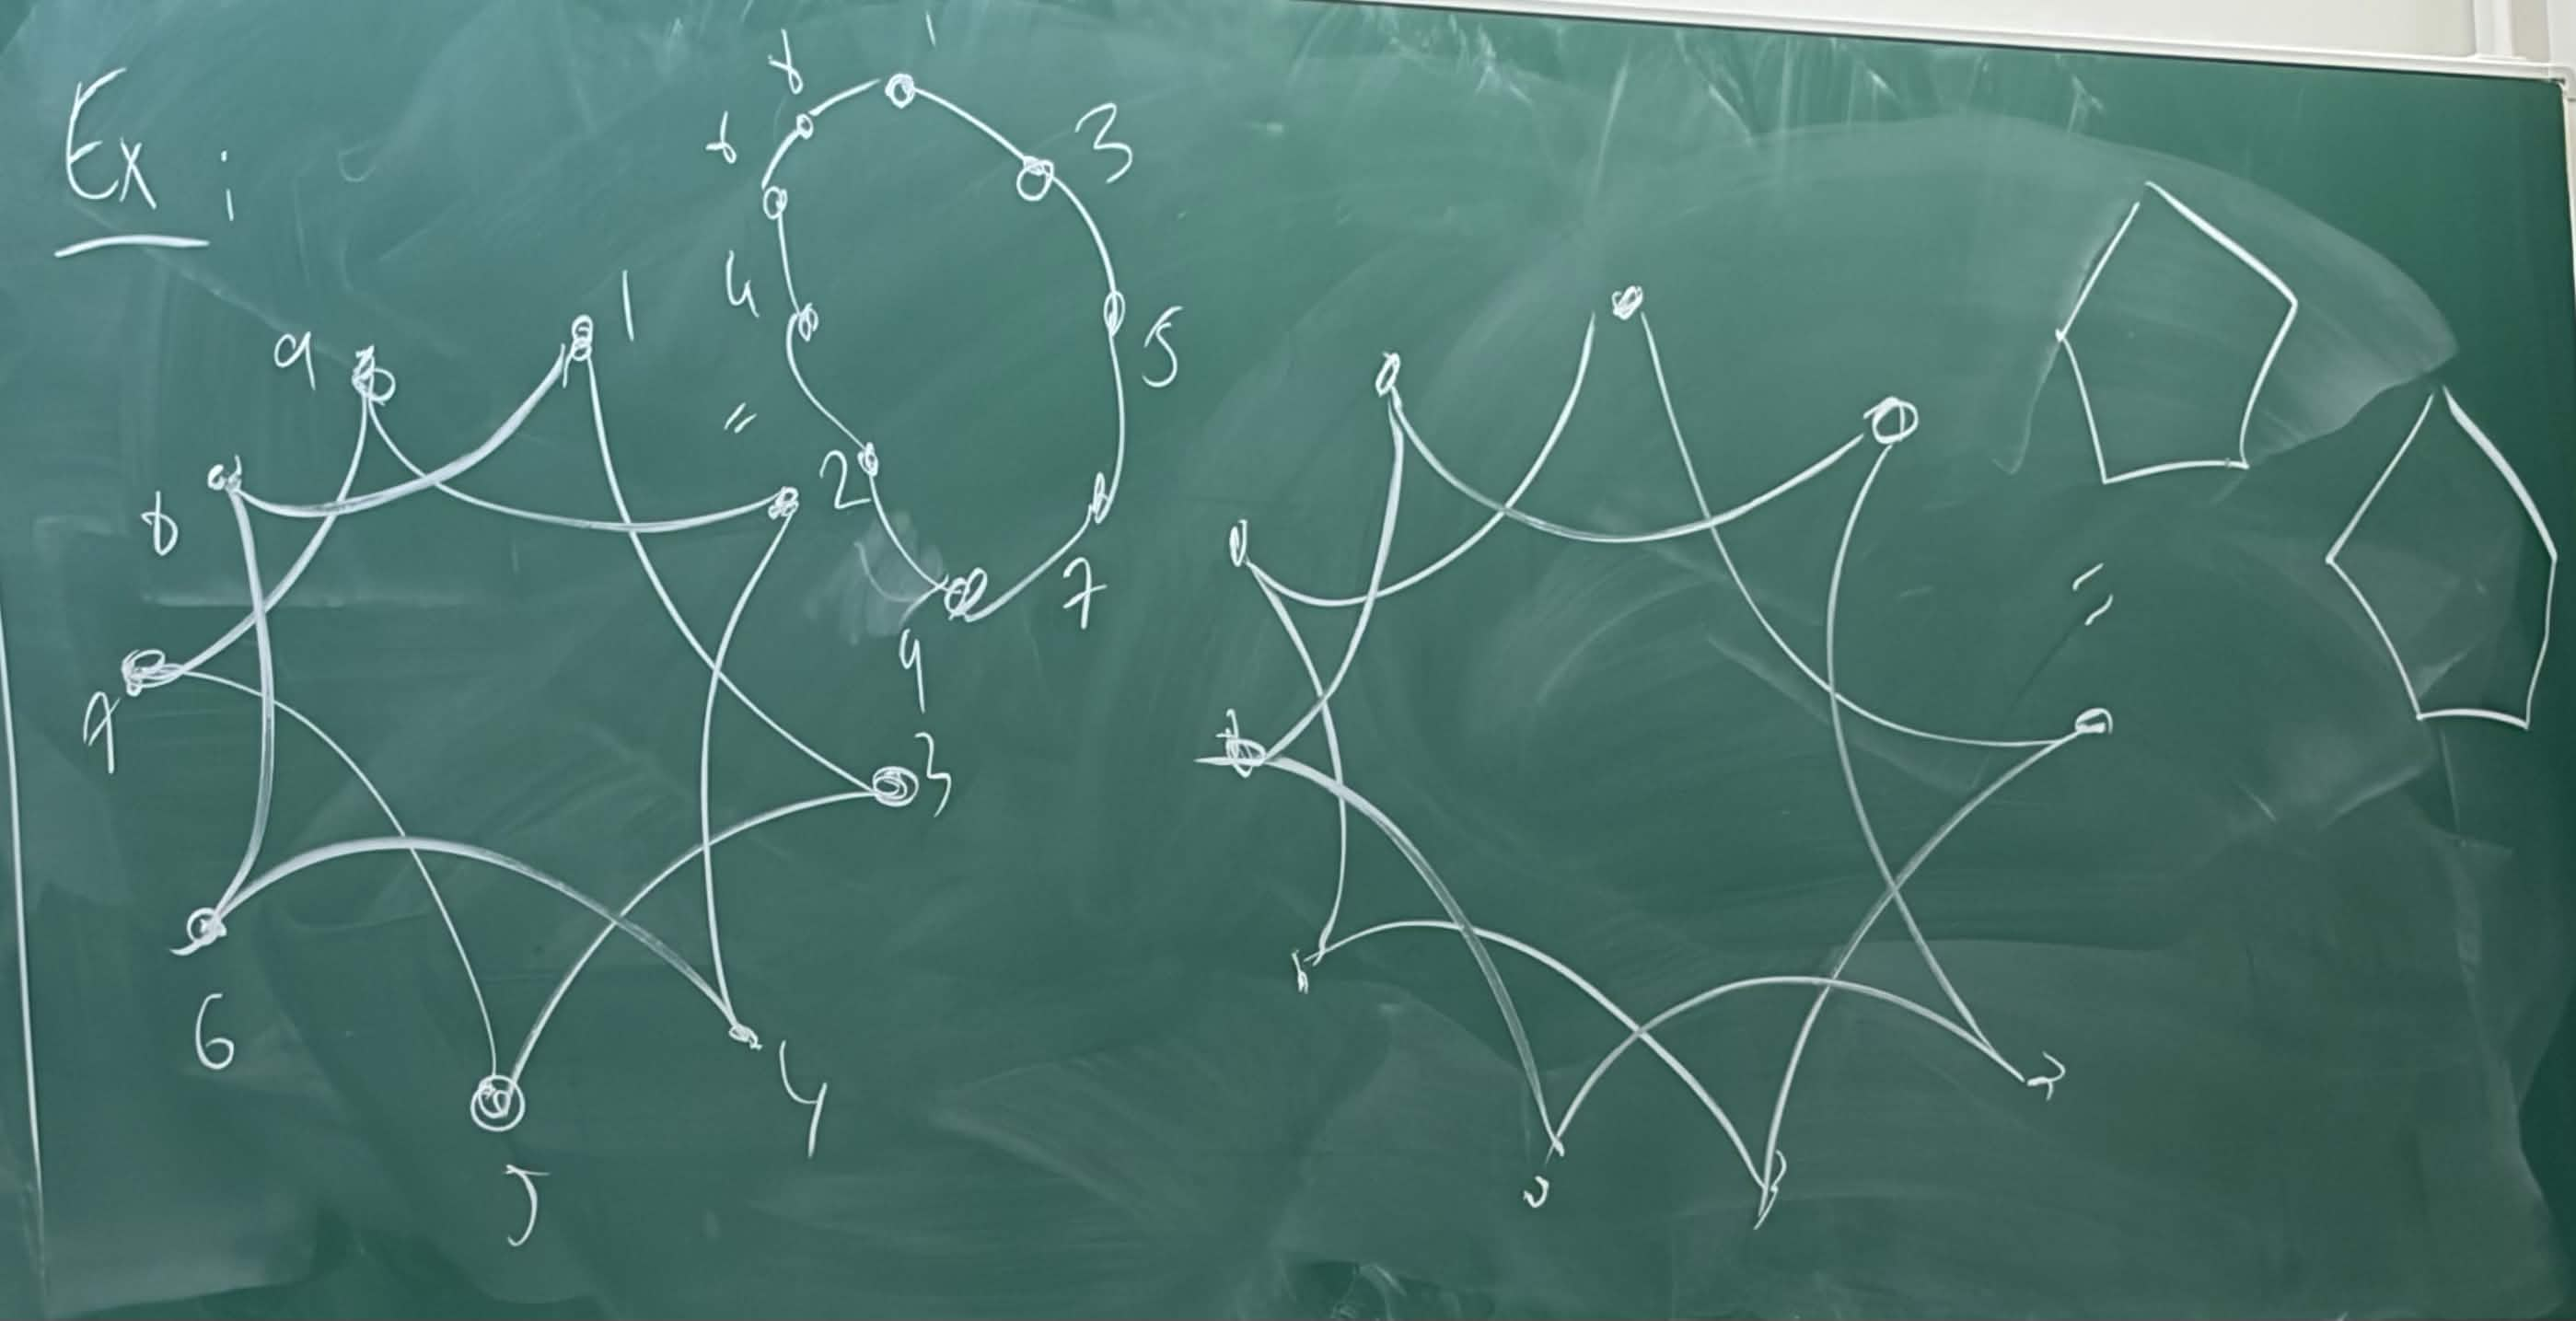
\includegraphics[width=0.7\textwidth]{./Figures/Connectivity.jpg}
    \caption{An example of connectivity (left one is connected but right one not)}
\end{figure}

\begin{question}
    How can we identify the connected components of a graph?
\end{question}

\begin{algorithm}[H] \label{alg: find component}
    \caption{Find the connected component containing \(v\)}
    \SetKwInput{KwInput}{Input}
    \SetKwInput{KwOutput}{Output}
    \KwInput{A graph \(G = (V, E)\) and a vertex \(v \in V\)}
    \KwOutput{Connected component \(C \subseteq V\) s.t. \(v \in C\)}
    \DontPrintSemicolon
    \Comment*[l]{We will maintain two sets of vertices. Let \(W\) be the component so far, i.e. vertices we can reach from \(v\) whose neighborhood we have explored.}
    Initially \(W_0 = \varnothing \).
    \(Q_0 = \left\{ v \right\} \). \Comment*[l]{\(Q=\)queue of vertices to explore} 
    \For() {the \(i\)-th step} {
        \If() {\(Q_{i-1} = \varnothing \)} {
            DONE. Return \(W\) as the component as \(v\).  
        }
        \Else() {
            Let \(w\) be an arbitrary vertex in \(Q_{i-1}\). 
            \(Q_i = Q_{i-1} \setminus \left\{ w \right\} \), \(W_i = W_{i-1} \cup \left\{ w \right\} \). 

            Explore the neighborhood of \(w\): If \(u\) is a neighborhood of \(w\) and \(u \notin Q \cup W_i\), then add it to \(Q_i\).         
        }
    } 
\end{algorithm}

\begin{claim}
    The algorithm is finite.
\end{claim}
\begin{explanation}
    In every step, if we are not done, we add a distinct item to \(W\) (since \(Q_i\) and \(W_i\) are disjoint) and never remove it. Thus, we do at most \(\vert V(G) \vert \) steps.  
\end{explanation}

\begin{claim}
    The algorithm is correct.
\end{claim}

\begin{explanation}
    Let \(C_v\) be the component of \(v\) and \(W\) be the output of the algorithm. We show that \(C_v = W\). We first show that \(W \subseteq C_v\). Prove by induction on number of steps that we only add something to \(W\) if it was in \(Q\). Also, we only add something to \(Q\) if it was a neighbor of an earlier member of \(W\). By induction, there is a path from this vertex to \(v\). Now we show \(C_v \subseteq W\). Suppose not, then let \(x \in C_v \setminus W\). Then there exists \(vx\)-path in \(G\), say \(v = v_0 v_1 v_2 \dots v_t = x \). Let \(j\) be the smallest index s.t. \(v_j \notin W\). Then \(v_{j-1}\) is in \(W\). Thus, we have explored its neighborhoods, so it would be in \(W\).                     
\end{explanation}

It would be nice to not only know the components of \(v\), but also paths that get there from \(v\). Thus, in the algorithm, when exploring the neighborhood of a vertex \(w \in Q_{i-1}\), if we add a neighbor \(u\) to \(Q_{i-1}\), we keep track of the edge \(\left\{ w, u \right\} \) that was used to reach \(u\). 

\begin{eg}
    Now if \(v = 4\) and the graph is the following figure: 
    \begin{figure}[H]
        \centering
        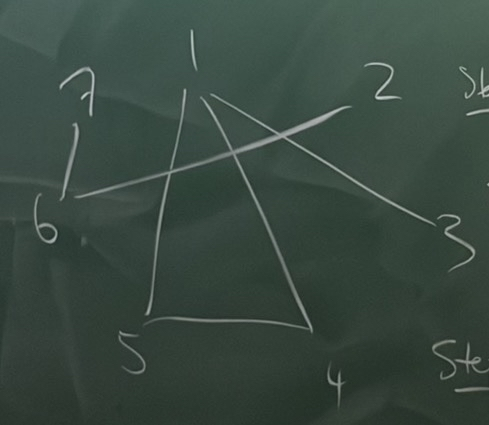
\includegraphics[width=0.4\textwidth]{./Figures/FindComponentsEx.png}
    \end{figure}
    Then we know 
    \begin{itemize}
        \item Step 0: \(Q_0 = \left\{ 4 \right\} \), \(W_0 = \left\{  \right\} \). 
        \item Step 1: \(w = 4\), \(Q_1 = \left\{ 1 (\left\{ 1, 4 \right\}), 5 (\left\{ 4, 5 \right\} ) \right\}   \), and \(W_1 = \left\{ 4 \right\} \). 
        \item Step 2: \(w = 1, Q_2 = \left\{ 5(\left\{ 4, 5 \right\} ), 3(\left\{ 1, 3 \right\} ) \right\} \), and \(W_2 = \left\{ 4, 1(\left\{ 1, 4 \right\} ) \right\} \). 
        \item Step 3: \(w = 5, Q_3 = \left\{ 3(\left\{ 1, 3 \right\} ) \right\} \), and \(W_3 = \left\{ 4, 1(\left\{ 1, 4 \right\} ), 5(\left\{ 4, 5 \right\} ) \right\} \). 
        \item Step 4: \(w = 3, Q_4 = \left\{  \right\},  \) and \(W_4 = \left\{ 4, 1(\left\{ 1, 4 \right\} ), 5(\left\{ 4, 5 \right\} ), 3(\left\{ 1, 3 \right\} ) \right\} \).           
    \end{itemize} 
\end{eg}

\begin{definition}
    A tree is a minimally connected graph, i.e. it is connected, but removing any edge disconnect it.
\end{definition}

\begin{proposition}
    Let \(T\) be an \(n\)-vertex graph. The following is equivalent: 
    \begin{itemize}
        \item [(1)] \(T\) is a tree. 
        \item [(2)] \(T\) is maximally acyclic. 
        \item [(3)] \(T\) is connected and has \(n - 1\) edges. 
        \item [(4)] \(T\) is acyclic and has \(n - 1\) edges.     
    \end{itemize}  
\end{proposition}

\begin{remark}
    Acyclic means no cycle.
\end{remark}
